\documentclass[10pt,conference,compsocconf]{IEEEtran}

\usepackage{hyperref}
\usepackage{graphicx}	% For figure environment


\begin{document}
\title{The Higgs challenge: A Machine Learning Practice Opportunity}

\author{
	Louis \textsc{Bettens}, Louis \textsc{Gounot}, Xavier \textsc{Nal}
}

\maketitle

\begin{abstract}
	In order to make sense of the increasing amounts of data produced by contemporary scientific advances, the assistance of computers and advances statistical techniques has become necessary.
	The field of machine learning consists of the study and use of algorithms that have the ability to find and recognize patterns hidden in vast amounts of data, and use them to make accurate predictions.
	This paper attempts to apply basic machine learning techniques to a dataset collected at CERN as part of a physics experiment.
\end{abstract}

\section{Introduction}

\section{Data cleaning and normalisation}
\label{sec:data-cleaning}

Since data in the real world comes in various formats and conventions, it makes sense to examine the representation of the input data to try to adapt it to the algorithms and programs we intend to use.
The first clean-up we applied to the data is to make sure that missing data was represented using a not-a-number value rather that a sentinel value of -999 as was the convention in the original dataset.
\cite{higgsml14}
While this convention is unambiguous in itself, it can hurt the accuracy of algorithm if they try to treat it as a meaningful datapoint.

The next step was to normalise the distribution of each feature by applying an affine transformation to bring the mean to 0 and the standard derivation to 1. This is common practice in machine learning since it allows to give equal weight to every feature in the eyes of distance functions.

To account for outliers, we then removed any data point that had any feature located more than 4 standard derivations away from the mean. This removes 5.01\% of data points.

\section{Exploratory data analysis}
In order to gather some insights as to how the data is structured, we first conducted a data exploration phase by plotting features together 2-by-2.
We used the Bokeh data visualisation library in a Jupyter notebook that is provided alongside our code.

Our overall insight is that both classes have distinct but overlapping distribution. For example in figure \ref{f1-f20}, we can see that the orange class tends to be higher on feature 1 than the blue class, although both classes harbor counterexamples by this metric. Given that all pairs of features on their own show ambiguity, we expect that the logistic regression method might perform better since it can take that ambiguity into account. We also noticed that feature 22 only takes 4 distinct discrete values, for example on figure \ref{f2-f22} Since perceptron-based classification algorithms might not have the ability to derive a good decision boundary in some cases with discrete, enumerated values, we decided to split this feature into 4 boolean features, each indicating one of the 4 distinct raw values of feature 22.

\section{Feature processing}
We add a feature of constant nonzero value to create a homogenous coordinate systems that allows perceptron-based algorithm to avoid sticking to the center of the coordinate system.

As mentioned before, we remove the 22nd feature, and add 4 boolean features that encode each of its discrete values.
\section{Algorithm selection}
We explored two algorithms: logistic regression, and ridge regression with polynomial feature extension. We split our training dataset into a test dataset proper (80\%) and validation dataset (20\%) to tune hyperparameters.
\section{Results}
Our best performing algorithm both on the validation dataset and in the competition was ridge regression with $lambda = 10^{-4}$ and polynomial expansion up to degree 7.
\section{Conclusion}

\begin{figure}
	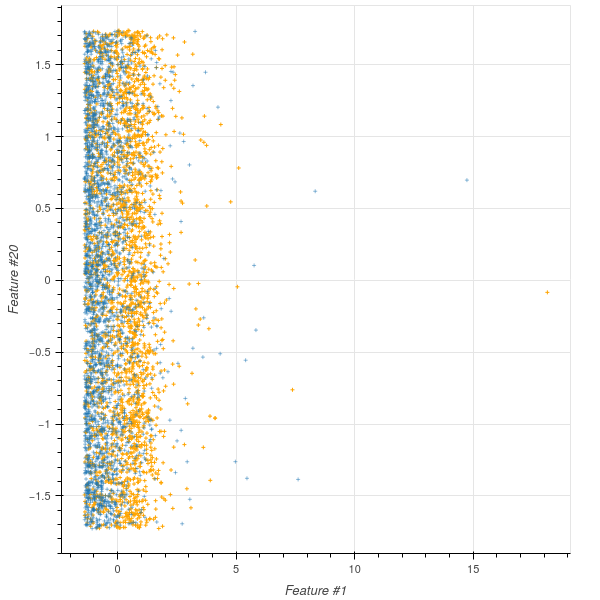
\includegraphics[width=\columnwidth]{f1-f20.png}
	\caption{Example plot of Features 1 and 20}
	\label{f1-f20}
\end{figure}

\begin{figure}
	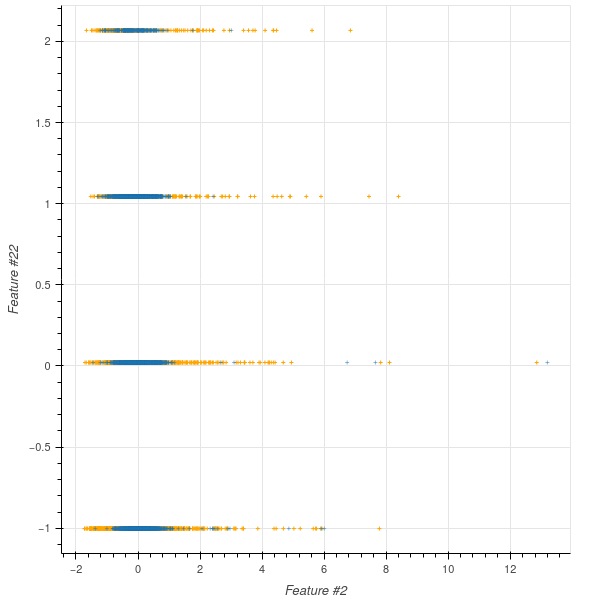
\includegraphics[width=\columnwidth]{f2-f22.png}
	\caption{Example plot of Features 2 and 22}
	\label{f2-f22}
\end{figure}

\bibliographystyle{IEEEtran}
\bibliography{literature}

\end{document}
